\scanpage{101}
\mspage{18}
\margin{De plus, il y a lieu d'exiger \unsure{1°} que $\Theta$ soit trivial sur $I'\cap X'_K$, et qu'une puissance $\Theta^{\unsure{\nu K}}$ de $\Theta$ $(\nu\geq1)$ soit \unsure{triviale|trivial} 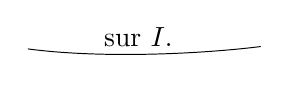
\begin{tikzpicture}[baseline=(surI.base),line cap=round]
\node[inner sep=0pt] (surI) at (0,0) {sur $I$.};
\draw[line width=.35pt] (-1.40,-.15)
 ..controls(-.50,-.27)and(.74,-.22)..(1.55,-.12);
\end{tikzpicture} Car $X'_K\ne\phi$ implique alors que $X'$ est $\unsure{+}$, $\unsure{=}$ connexe. \deleted{De plus}}

de $\Theta$ se relève en une action de $\Theta$ sur $\widehat{\Pi}_1(X',I')$, où $I'=X'\vert I$.
\deleted{$\unsure{\exists a'\in}$} $I'\cap X'_K\ne\phi$, $X'$ \unsure{étant|ét.} connexe (il suffit que $\Gamma$ soit transitif sur $\pi_0(X')$ i.e. que $X'$ soit ``$K$-connexe'' i.e. connexe en tant que schéma sur $K$) donc l'action remontée est unique.

\inserted{La condition 2 s'explicite en pratique comme une condition de stabilité de certains ss-groupes ouverts d'un $\pi_1(X,x)$ $(x\in X_K\cap I)$ sous l'action de $\pi$}

3) Sous les conditions de 2), pour tt hom $f:X'\longrightarrow Y$ et \deleted{tout}\inserted{un} $x'\in X'_K\cap I'$, \deleted{l'action} peut trouver le $\Theta'$ \deleted{\unsure{des tels}} de telle façon que l'autom. de $\widehat{\pi}_1(X',x')$ qu'il induit laisse stable le noyau de
\[
\widehat{\pi}_1(X',x)\mathrel{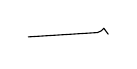
\begin{tikzpicture}[baseline=-.35ex,line cap=round,line join=round]
\draw[line width=.4pt] (0,0)--(.88,.055)
 ..controls(.92,.06)and(.94,.09)..(.96,.11)--(1.015,.035);
\end{tikzpicture}}\widehat{\pi}_1(Y,f(x)).
\]
C'est encore une condition de stabilité pour certains sous-groupes, mais pas néc. d'indice fini, de $\pi_1(X,x)$ par $\Theta$.

\margin{On peut \deleted{\unsure{généraliser}}\inserted{renforcer} cette condition, en \unsure{en supposant|ne supposant} \deleted{\unsure{tt|$\forall$}} \unsure{pas} $x'\in X'_K\cap I$, et en \deleted{\unsure{l'imposant}} exigeant que pour tt $\nu$ tel $\Theta'^\nu x'=x'$, $\Theta'^\nu$ sur $\pi_1(X',x')$, \unsure{préserve le noyau de} $f$ $\widehat{\pi}_1(Y,f(x'))$.}

4) Soient $X'_1,X'_2$ deux rev. étales finis de $X$, et $f$ un morphisme
\[
X'_1\xrightarrow{f}X'_2
\]
(\uuline{pas néc.} \uuline{un $X$-morphisme} !), $I'_1=X'_1\mathrel{\begin{tikzpicture}[baseline=-.50ex,line cap=round]
\draw[line width=.4pt] (0,-.17)--(0,.21);
\draw[line width=.4pt] (0,0)--(.10,.01);
\end{tikzpicture}} I$, $I'_2=X'_2\vert I$ on suppose \deleted{déjà que} que $J\overset{\mathrm{def}}=I'_1\cap f^{-1}(I'_2)\ne\phi$, \deleted{plus précisément que} \deleted{$\unsure{I'_1|X'_1}\cap f^{-1}(I'_2)\longrightarrow$} alors \deleted{le morph} le morphisme
\[
\Pi_1(X'_1,J)\longrightarrow\widehat{\Pi}_1(X'_2,I'_2)
\]
est compatible avec l'action 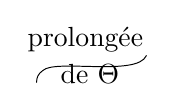
\begin{tikzpicture}[baseline=(deTheta.base),line cap=round]
\node[anchor=base west,inner sep=0pt] (deTheta) at (.27,0) {de $\Theta$};
\node[anchor=base west,inner sep=0pt] (prolongee) at (-.15,.46) {\inserted{prolongée}};
\draw[line width=.35pt] ([xshift=1pt,yshift=-1pt]prolongee.south east)
 ..controls(1.25,.08)and(.20,.31)..(.05,.16)
 ..controls(-.01,.12)and(-.03,.07)..(-.03,.01);
\end{tikzpicture} sur les groupoïdes (pour un choix compatible de cette action, s'il y a ambiguïté, cf 2°).
\mspage{100}
